\chapter{Etat de l'art}

\section{Différents types de données}
Pour réaliser notre projet : animer un modèle de main en se basant sur les mouvements de la main de l'utilisateur, nous avons à disposition une 
Kinect 2 et un LeapMotion. Pour commencer notre état de l'art, nous allons voir quelles données peuvent être récupérées par ces outils et 
quels autres moyens auraient pu être utilisés pour réaliser ce projet.\\

Une liste non exhaustive des périphériques et des données qu'ils fournissent : 
\begin{itemize}
  \item Kinect1 et Kinect 2 de Microsoft, fournissent, en données brutes, une image couleur ainsi qu'une image de profondeur. 
En utilisant le SDK fourni, on dispose en plus de nombreux outils parmi lesquels une détection du squelette et pour Kinect 2 
une abstraction de la main avec 4 points détectés : le centre du poignet, le centre de la main, le sommet du pouce et le sommet du majeur. 
  \item LeapMotion fournit, en données brutes, un squelette 3D plus détaillé mais sur une zone 
plus restreinte. Avec le SDK, on a accès directement à un squelette très détaillé de la main.
    \begin{figure}[!h]
    \center
    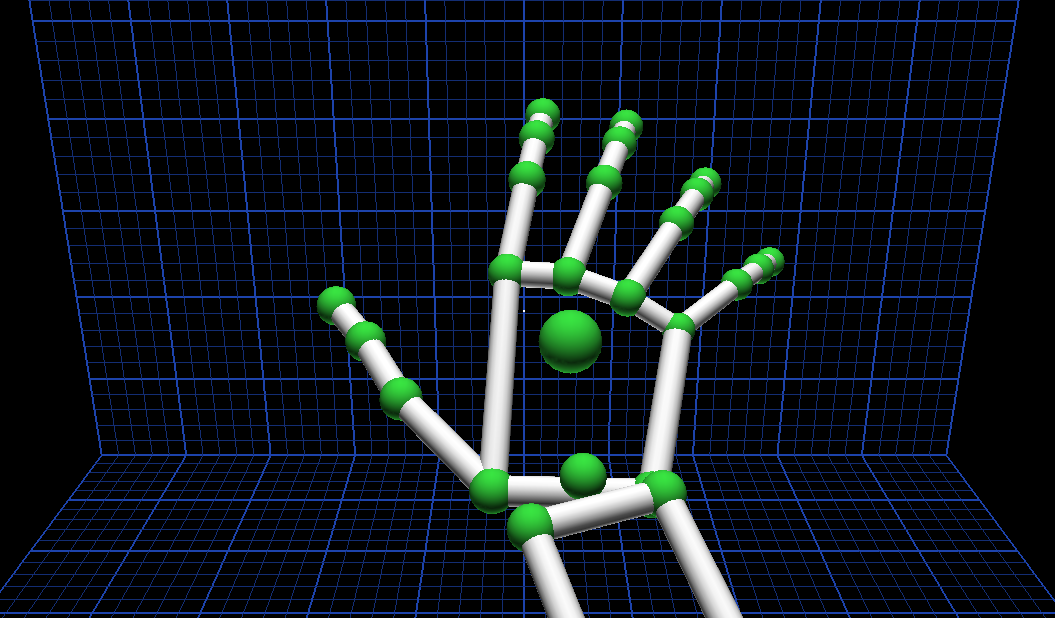
\includegraphics[width=350px]{images/SDK_LeapMotion.png}
    \caption{Squelette de la main de l'utilisateur détecté par la LeapMotion}
    \end{figure}
  \item RealSense est un périphérique relativement récent, à mi chemin entre Kinect 2 et LeapMotion. On peut, à l'aide du SDK fourni, récupérer des informations semblables à celles fournies par LeapMotion : 
  22 points de la main détectés et suivis
\end{itemize}
\ \\

On peut utiliser des outils spécifiques (Kinect) ou des caméras classiques pour obtenir des images couleurs.
Bien que possédant plus d'informations que les images de profondeur (3 canaux au lieu d'un), les images couleurs sont moins adaptées aux calculs 3D.\\

Ces données couleurs peuvent être utilisées avec des accessoires colorés pour simplifier la détection des points de la main \cite{wang2009real}.
Cette méthode permet de détecter plus facilement les jointures et les points d'intér\^{e}t. 
Cependant, cela ajoute des contraintes, notamment le fait de devoir porter un gant standardisé.\\

On associe également les données couleurs avec des données de profondeur pour améliorer la détection et gérer les cas de superposition \cite{van2011combining}.\\

L'autre type de données est la carte de profondeur, image en niveau de gris servant à représenter la profondeur. 
Cette carte de profondeur est utilisée par un grand nombre de méthodes pour les problèmes de clustering du corps humain, notamment les SDK de Kinect 1 et Kinect 2 se basent principalement dessus pour fournir le squelette \cite{export:145347}.
Les SDK de Kinect1/Kinect2 étant prévus pour le suivi du corps entier, ils sont peu performants pour le suivi précis de parties spécifiques (comme la main).
L'utilisation directe du SDK semble donc insuffisante pour résoudre notre problème. Cependant, on peut aussi récupérer les données brutes fournies par la Kinect 2 et certaines méthodes se contentent d'une image de profondeur pour la détection de la main \cite{export:238453}.

\section{Détection de la main}

La Kinect 2 possède deux types de caméra, une caméra couleur et une caméra de profondeur utilisant la méthode 
\og Time of Flight \fg. Les caméras de type \og Time of Flight \fg
récupérent les rayons envoyés par projecteur qui ont été réfléchis par les objets de la scène, ce qui permet d'obtenir les informations de profondeur. 
Il existe plusieurs solutions utilisant l'une ou l'autre de ces caméras. Nous allons
dans cette partie, détailler plusieurs méthodes réalisées jusqu'à maintenant.

\subsection{Détection et suivi de la main à partir d'une image couleur}
La méthode proposée par S. Bilal et al \cite{haarlike} utilise l'algorithme de Viola et Jones \cite{viola2001jones} afin
de détecter la main et fournir la position de celle-ci en créant une ROI (région d'intérêt) autour d'elle.
L'algorithme de Viola et Jones \cite{viola2001jones} nécessite une 
base de connaissances composée des caractéristiques de l'objet recherché. Elle est utilisée dans un 
apprentissage supervisé, c'est-à-dire que l'algorithme a besoin de données représentant
l'objet à détecter pour classifier les caractéristiques de celui-ci. Cet algorithme est basé sur des caractéristiques 
pseudo-Haar qui crée des masques rectangulaires et adjacents dans différentes zones de l'image (voir Fig. \ref{fig:pseudo_haar}). 
Chaque masque calcule l'intensité des pixels qu'il contient, puis l'algorithme fait la différence entre les masques blancs et 
les masques noirs.\\

\begin{figure}[!h]
\center
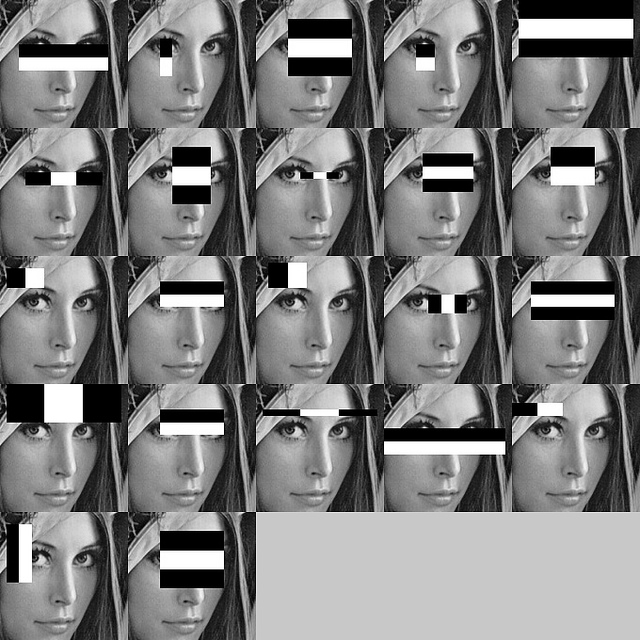
\includegraphics[width=200px]{images/pseudoHaar.jpg}
\caption{Exemple de caractéristiques pseudo-Haar utilisées pour l'algorithme Viola et Jones}
\label{fig:pseudo_haar}
\end{figure}

Pour améliorer les performances de leur algorithme, Viola et Jones utilisent la méthode Adaboost. Son
principe est de sélectionner les caractéristiques les plus performantes pour la détection de l'objet grâce à
un calcul de probabilité utilisant l'entropie\footnote{valeur mesurant l'incertitude} des données.\\

Une fois qu'une ROI est formée autour de la main de l'utilisateur, S. Bilal et al \cite{haarlike} changent d'espace colorimétrique
afin de pouvoir différencier la main du reste de l'environnement. Pour cela, ils choisissent 
d'utiliser l'espace YCbCr qui permet d'obtenir des informations de chromaticité dont la valeur est presque équivalente
quelle que soit la couleur de peau de l'utilisateur \cite{yoo1999fast}. Dès que la ROI de la main est binarisée, il est possible
de détecter le bout des doigts. Il faut tout d'abord calculer le centroïde de la forme de la main, puis la distance entre
ce centroïde et chaque point du contour de la main. Le contour d'une forme dans une image est défini par un changement brutal
de couleur. Cette méthode permet d'obtenir un graphe correspondant à la Fig. \ref{fig:handHisto}, où chaque pic représente un doigt.\\

\begin{figure}[!h]
\center
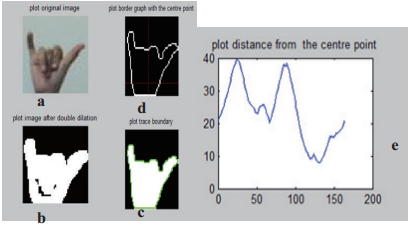
\includegraphics[width=300px]{images/handHisto.png}
\caption{Histogramme des distances entre les points du contour de la main et le centroide}
\label{fig:handHisto}
\end{figure}

Afin de pouvoir suivre la main, S. Bilal et al \cite{haarlike} utilisent l'algorithme de Kalman \cite{kalman}.
Cet algorithme permet de prédire la position d'un objet, ce qui va permettre de suivre la main malgré
le bruit présent dans l'image. De plus, cette méthode n'a besoin de connaître que l'état précédent à celui 
qui est calculé. Etant donné que l'algorithme de Kalman est un algorithme de prédiction, il peut ne pas être très
précis lorsque l'utilisateur effectue des changements de direction rapides avec sa main.\\

Cette méthode nous permet de déterminer la position de la main et de détecter le bout des doigts. Cependant, elle ne nous permet
pas de réaliser notre projet entièrement. En effet, nous avons besoin de plus de précisions en détectant les articulations
de la main. De plus, cette méthode est sensible à la luminosité de la scène filmée et n'est pas très adaptée
à la modélisation 3D d'une main.

\subsection{Détection et suivi de la main à partir d'une image de profondeur}
Une seconde solution utilise une image de profondeur plutôt que l'image binarisée avec le changement d'espace colorimétrique.
Pour réaliser la détection de la main, il faut dans un premier temps déterminer une ROI
autour de celle-ci.\\ 

Cette première étape a été expliquée par Sharp et al \cite{export:238453}, qui utilisent un classifieur
basé sur la méthode développée par J. Shotton et al \cite{export:145347}. Ce classifieur permet d'effectuer de la reconnaissance
des parties du corps et permet également de détecter les articulations. Dans ce but, cette méthode utilise l'algorithme de Lepetit et al
\cite{lepetit2005randomized} qui crée un arbre de décision à partir des données d'entraînement et descend dans celui-ci
jusqu'à atteindre une feuille (voir Fig. \ref{fig:arbre}).\\

\begin{figure}[!h]
   \begin{center}
     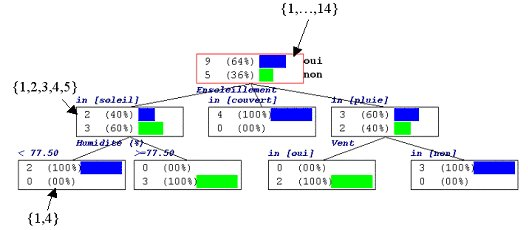
\includegraphics[width=10cm]{images/Arbre_de_decision.jpg}
     \caption{Exemple d'arbre de décision}
     \label{fig:arbre}
   \end{center}
 \end{figure} 
 
Les feuilles de cet arbre sont les différentes parties du corps à reconnaître. Cet arbre est construit en calculant
l'entropie de chaque pixel, ce qui permet de déterminer à quelle partie du corps il appartient.\\

\begin{figure}[!h]
 \begin{center}
  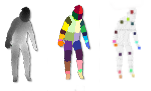
\includegraphics[width=300px]{images/bodyrecognition.png}
  \caption{Résultat de la détection des parties du corps et des articulations grâce à la méthode de \cite{export:145347}}
  \label{fig:bodyrecognition}
 \end{center}
\end{figure}

On voit dans la Fig. \ref{fig:bodyrecognition} que l'articulation de la main est détectée, il est alors possible de construire
une ROI autour de ce point. Cette méthode a été implémentée dans la caméra Kinect.\\

La méthode utilisée dans \cite{export:238453} ne nécessite aucune donnée provenant d'images antérieures. L'ensemble
des calculs sont réalisés sur une image à partir d'une base d'apprentissage contenant différentes postures de la
main. Etant donné qu'il est impossible de stocker toutes les postures de la main, la méthode de T. Sharp et al \cite{export:238453}
calcule une fonction énergie permettant de déterminer quelle est la posture la plus représentative de celle de la main
de l'utilisateur. Cette fonction énergie est calculée à partir des pixels du modèle et ceux de l'image de profondeur
capturée par la caméra. Elle est définie par le calcul suivant :
\begin{equation}
 E^{au}(Z_{roi}, R_{roi}) = \sum_{ij} \bar{\rho(z_{ij}} - r_{ij})
\end{equation}
Dans cette équation, $z_{ij}$ représente le pixel à la position (i,j) dans le modèle et $r_{ij}$ représente le pixel à la position (i,j)
provenant de l'image de profondeur. La fonction $\rho(e)$, quant à elle, est équivalente à $min(|e|,\tau)$ où $\tau$ est une valeur fixe permettant d'éliminer le bruit présent dans l'image de profondeur.

\section{Modélisation 3D de la main}
%input
Pour mieux visualiser les actions réalisées par la main de l'utilisateur et pour faire correspondre les jointures détectées au modèle, il est nécessaire d'avoir
un modèle de la main qui soit réaliste et précis par rapport à la réalité. Pour cela, nous avons besoin d'un
maillage d'une main modèle que nous allons ensuite adapter à la main de l'utilisateur.\\

%icp
La méthode utilisée par J. Taylor et al \cite{export:217428} permet en utilisant l'algorithme
ICP\footnote{Iterated Closest Point} \cite{121791} de modifier le maillage de la main afin
que les points de celui-ci aient une distance moins importante avec le nuage de points fourni par la 
caméra. Pour cela, l'algorithme ICP recherche les transformations, rotation et translation, qui permettent 
à partir d'un maillage M d'obtenir un maillage P. Dans notre cas, le maillage M représente le modèle de main donné en entrée
et le maillage P représente la main de l'utilisateur. ICP fonctionne en quatre étapes distinctes.
\begin{itemize}
  \item Associer les points grâce aux critères du plus proche voisin. Pour cela, il suffit de calculer la distance euclidienne d'un
   point avec tous les autres points qui font partis du balayage que nous voulons comparer et de prendre la distance la plus petite.
  \item Estimer la transformation des points grâce à une fonction d'erreur quadratique moyenne, permettant ainsi de trouver la meilleure
  transformation possible.
  \item Effectuer la transformation du nuage de points ayant la plus petite erreur.
  \item Itérer jusqu'à ce qu'on ait atteint la condition de fin fixée par l'utilisateur.
\end{itemize} 
\ \\

%squelette
La méthode de J. Taylor et al \cite{export:217428} permet également d'adapter le squelette du modèle de la 
main, ce qui permet d'obtenir une précision plus importante lors de l'utilisation de l'application.
Pour cela, on applique à chaque os du squelette du modèle d'origine, 
une transformation ( rotation et forme) qui dépend de celle calculée dans la phase précédente.\\

%Surface
Ensuite, la méthode recalcule la surface à partir du nouveaux maillage et du nouveau squelette.
\begin{itemize}
\item Si la surface est paramétrée par un ensemble de points de contrôle, comme un polyèdre
ou une surface de subdivision, on applique une fonction surface pour retrouver le point de l'espace correspondant.
\item Si le maillage est composé de triangles, on applique la fonction au point résultant de interpolation linéaire entre les sommets des triangles.\\
\end{itemize}

%Optimisation
Entre chaque opération, on applique une fonction de minimisation d'énergie,
on obtient alors une convergence des résultats plus rapide qu'en utilisant simplement ICP une fois.

\section{Evaluation des solutions envisagées}
Parmi les solutions que nous avons envisagées dans cet état de l'art, nous avons vu que la solution avec une 
image couleur pouvait être limitée. Celle-ci nécessite un algorithme permettant de suivre au mieux
la main de l'utilisateur. L'algorithme de Kalman est efficace, mais peu précis lors de changements d'orientation
brusques et il est également assez complexe à mettre en place. Il existe d'autres méthodes de suivi qui sont
peut-être plus appropriées à la conception d'une nouvelle IHM, mais le suivi n'est pas le seul défaut de cette
méthode pour la réalisation de notre projet. Une 
modélisation 3D de la main n'est pas possible avec ce genre de méthode. En effet, sans l'information de 
profondeur de la main, il est difficile de déterminer de nombreuses postures de celle-ci. Cette solution était une première approche de la 
détection de la main ainsi que des doigts qui reste efficace avec une luminosité correcte.\\

Notre choix pour la réalisation de ce projet se dirige plutôt vers l'utilisation de la caméra de profondeur.
La Kinect 2 ayant déjà une implémentation d'une partie des étapes permettant la réalisation de notre projet, nous pourrons
nous concentrer sur la partie plus spécifique de détection et de localisation des articulations de la main. 
Pour cela, nous avons vu que la méthode utilisant l'image de profondeur pouvait être efficace grâce à la 
détermination de la posture de la main. Cela nous permet ainsi d'ajuster un modèle de main et de fabriquer
le squelette en fonction de ce modèle.\\
